\subsection{Cross Talk}

The distance between anode channels is very short,
so the influence of mutual capacitance become large
and this capacitive coupling induce cross talk noise.
This effect notably appears the channel where the differnce of the charge between adjacents channels is large, such as the channel around stopped point of proton.
Figure\ref{fig:cross_talk1} shows the signal wave form of stopped channel and the front channel of typical proton event.
The signal wave form of stopped channel is differencial form of the one of the front channel.
This shape is appeared at channel number 1 which cannot enter drifted ionization electron in electric power lines.
These facts show the exisitence of cross talk.
Then, we implement this crosstalk phenomenon in Monte Carlo Simulation
by adding bipolar shape of the signal gaussian shape at adjacent channels.
The area of the mountain of cross talk bipolar shape is 10.5\% of the area of signal gaussian at each adjacent channel.
The value of 10.5\% is determined by comparing the distribuntion of integrated ADC at stopped channel between DATA and MC.
Figure\ref{fig:cross_talk2} shows integrated ADC distribution of stopped channel.
Black is DATA and blue is simulation with cross talk red is simulation without cross talk.
As this figure shows, DATA and MC with cross talk is good agreement,
and the value of 10.5\% is reasonable.

\begin{figure}[htbp]
  \begin{tabular}{cc}
    \begin{minipage}{0.5\hsize}
      \centering
      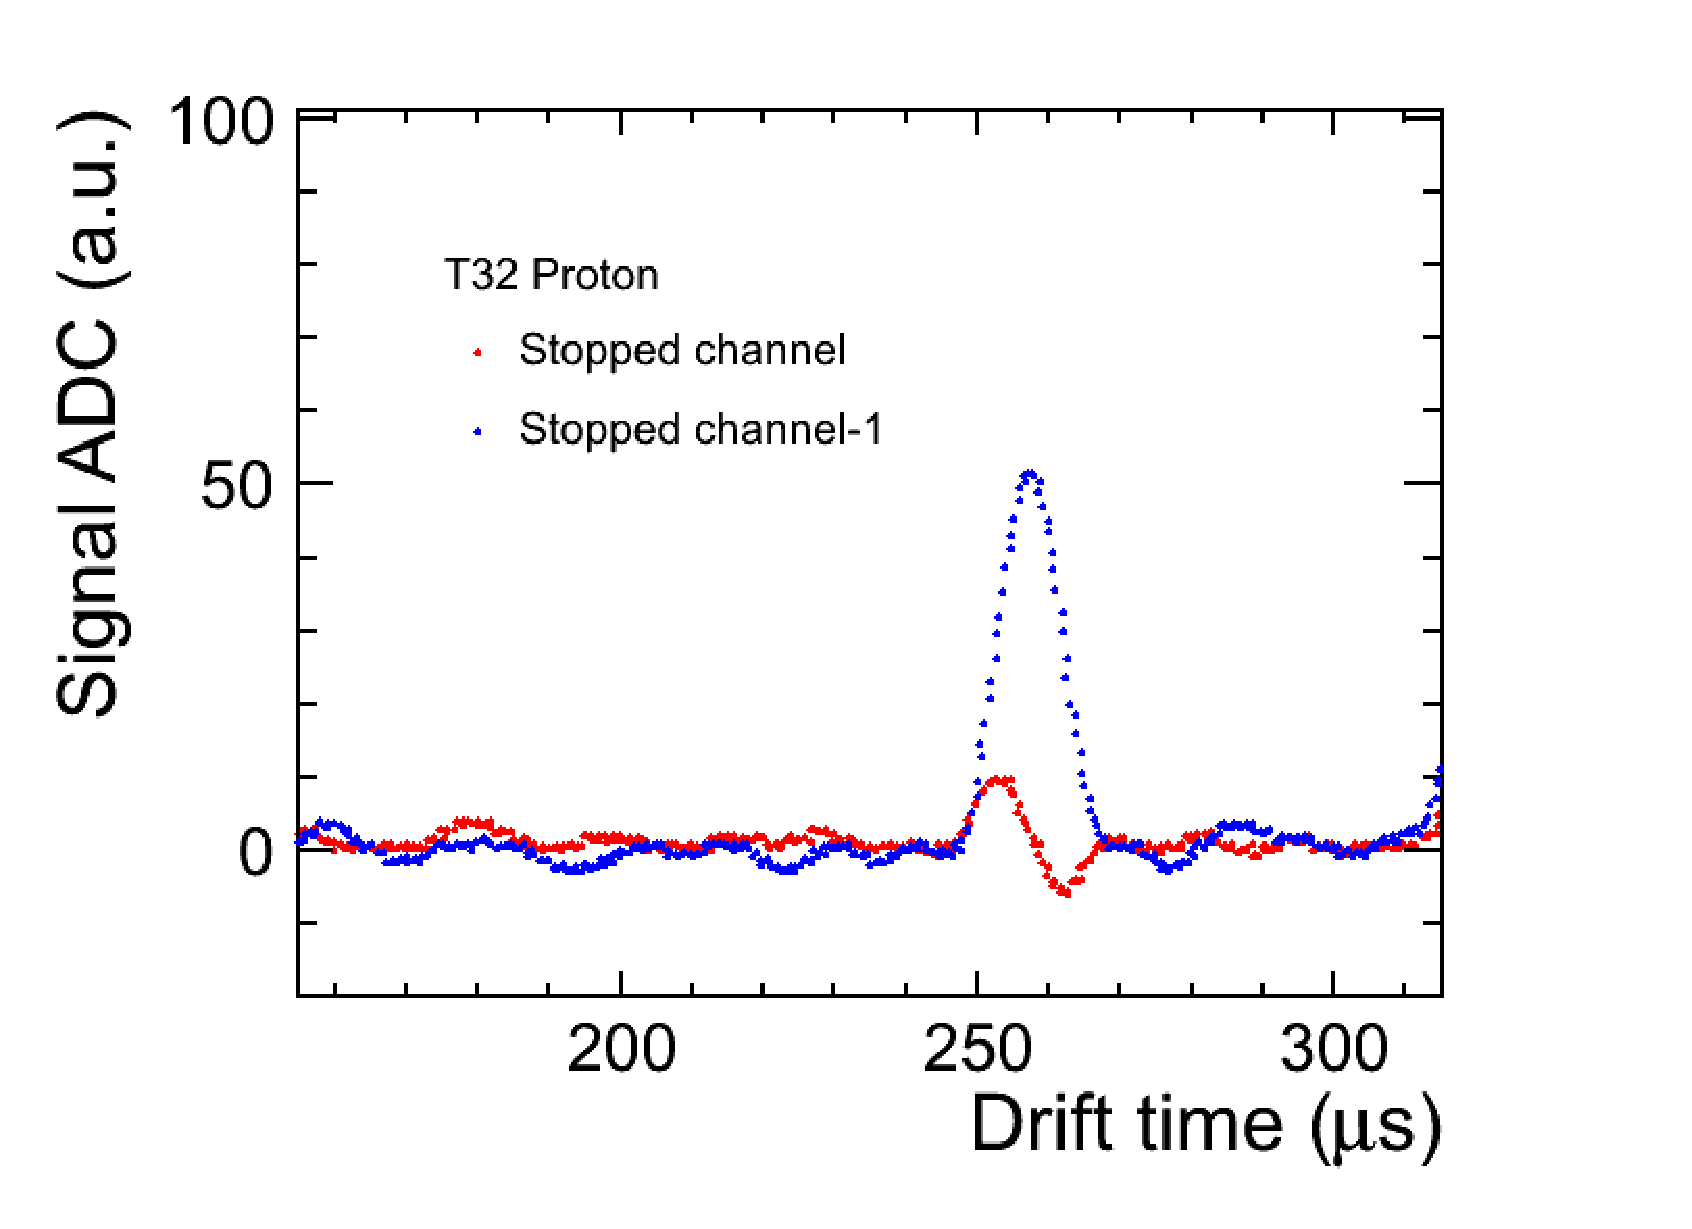
\includegraphics[width=6cm,clip]{fig/cross_talk_1.eps}
      \caption{Signal wave form of stopped channel and the front channel}
      \label{fig:cross_talk1}
    \end{minipage}
    \begin{minipage}{0.5\hsize}
      \centering
      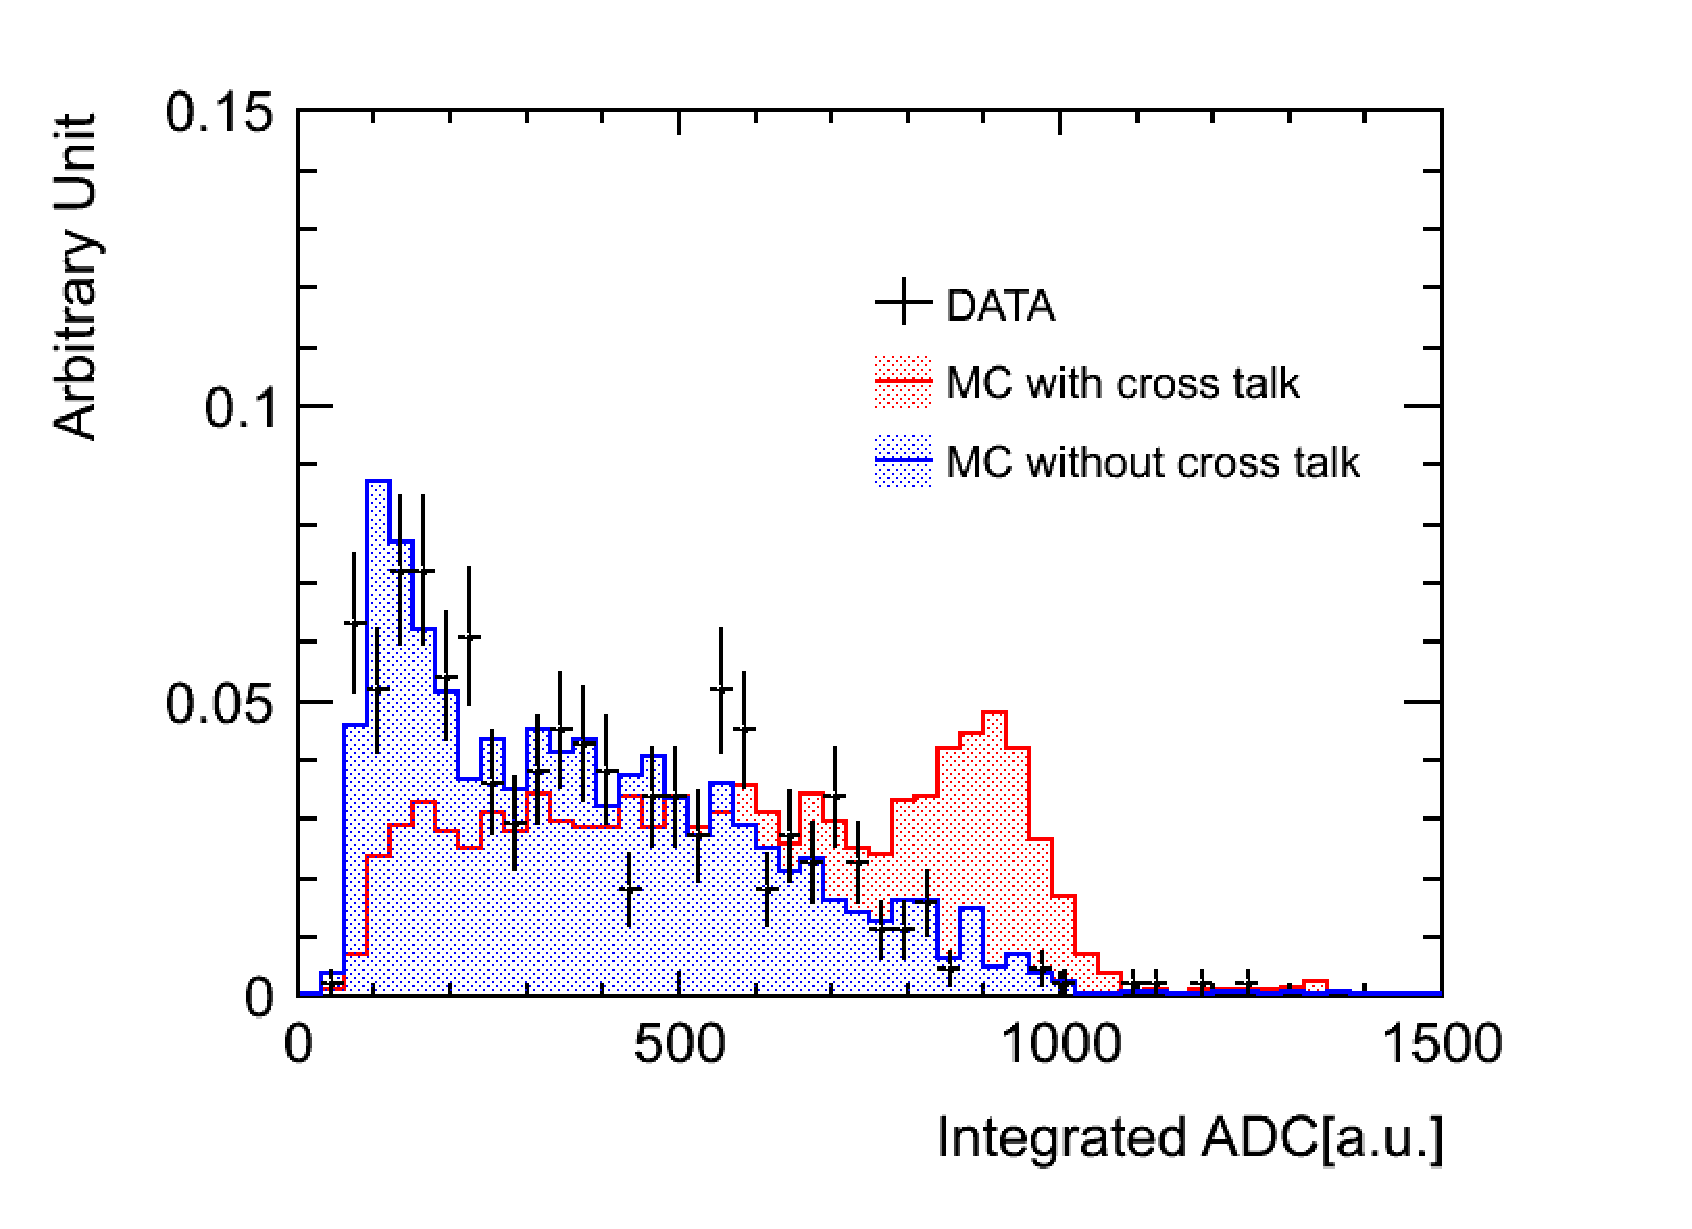
\includegraphics[width=6cm,clip]{fig/cross_talk_2.eps}
      \caption{Integrated ADC distribution of stopped channel}
      \label{fig:cross_talk2}
    \end{minipage}
  \end{tabular}
\end{figure}


